\documentclass{beamer}
%\documentclass[aspectratio=169]{beamer}
%
\mode<presentation>
{
  \usetheme{default}      
  \usecolortheme{default}
  \usefonttheme{default} 
  \setbeamertemplate{navigation symbols}{}
  \setbeamertemplate{caption}[numbered]
} 

\usepackage[english]{babel}
\usepackage[utf8x]{inputenc}
\usepackage{bbm}
\usepackage{bm}

\newcommand{\1}[1]{\mathbbm{1}\left[#1\right]}
\newcommand{\norm}[1]{\left\lVert#1\right\rVert}
\newcommand{\yi}{y^{(i)}}
\newcommand{\yhat}{\hat{y}}
\newcommand{\yhati}{\hat{y}^{(i)}}
\newcommand{\bx}{\bm{x}}
\newcommand{\bxi}{\bx^{(i)}}
\newcommand{\pv}{\pause\vfill}
\newcommand{\p}{\pause}
\newcommand{\f}{\vfill}

\title{Machine learning from scratch}
\subtitle{Lecture 9: Conclusion (and some deep learning)}
\author{Alexis Zubiolo\newline\texttt{alexis.zubiolo@gmail.com}}
\institute{Data Science Team Lead @ Adcash}
\date{March 30, 2017}

\begin{document}

\begin{frame}
  \titlepage
\end{frame}

\begin{frame}{Course outline}
This is our last lecture.
\pv
Today we'll conclude, and talk a bit about \textbf{neural networks}.
\end{frame}

\begin{frame}
\begin{center}
\Huge{Neural networks}
\end{center}
\end{frame}

\begin{frame}{Neuron}
\begin{figure}
\centering
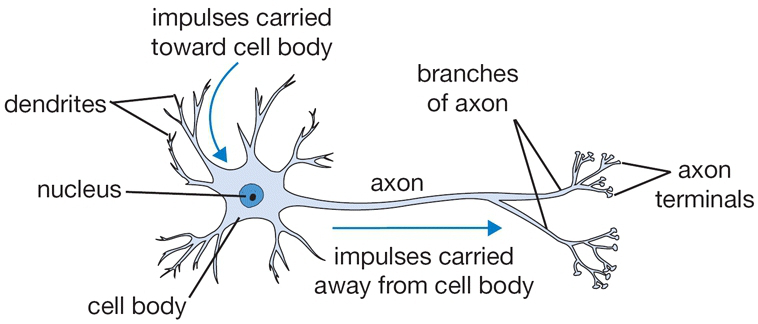
\includegraphics[width=\textwidth]{images/neuron.png}
\end{figure}
\end{frame}

\begin{frame}{Neuron (mathematical model)}
Neural networks are trying to model the logic:
\begin{figure}
\centering
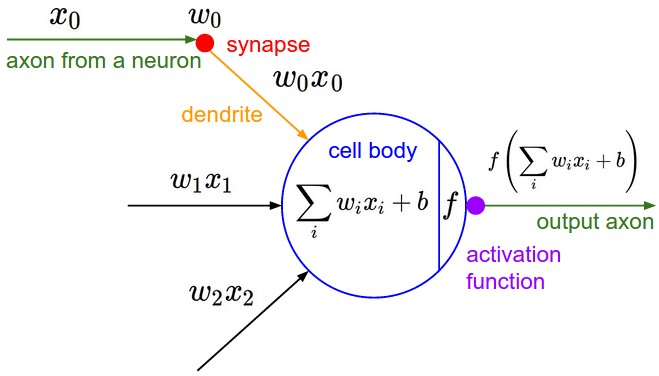
\includegraphics[width=\textwidth]{images/neuron_model.jpeg}
\end{figure}
\end{frame}

\begin{frame}{Single neuron case}
The neuron we've described performs the same task as the linear ML models we've seen previously:
\begin{itemize}
	\item Take an input $\bx$
	\item Compute the output $\theta^T\bx$
	\item Compare the output to the actual label $y$
\end{itemize}
\pv
A neural network will consist in \textbf{stacking layers} of neurons in order to build more complex models.
\end{frame}

\begin{frame}{Stacking neuron layers}
There are 3 types of \textbf{neuron layers}:
\begin{itemize}
	\item \textbf{Input layer} (which corresponds to $\bx$)
	\item \textbf{Output layer} (which correspond to $\yhat$)
	\item \textbf{Hidden layers} (layers between the input and output layers)
\end{itemize}
\pv
\begin{figure}
\centering
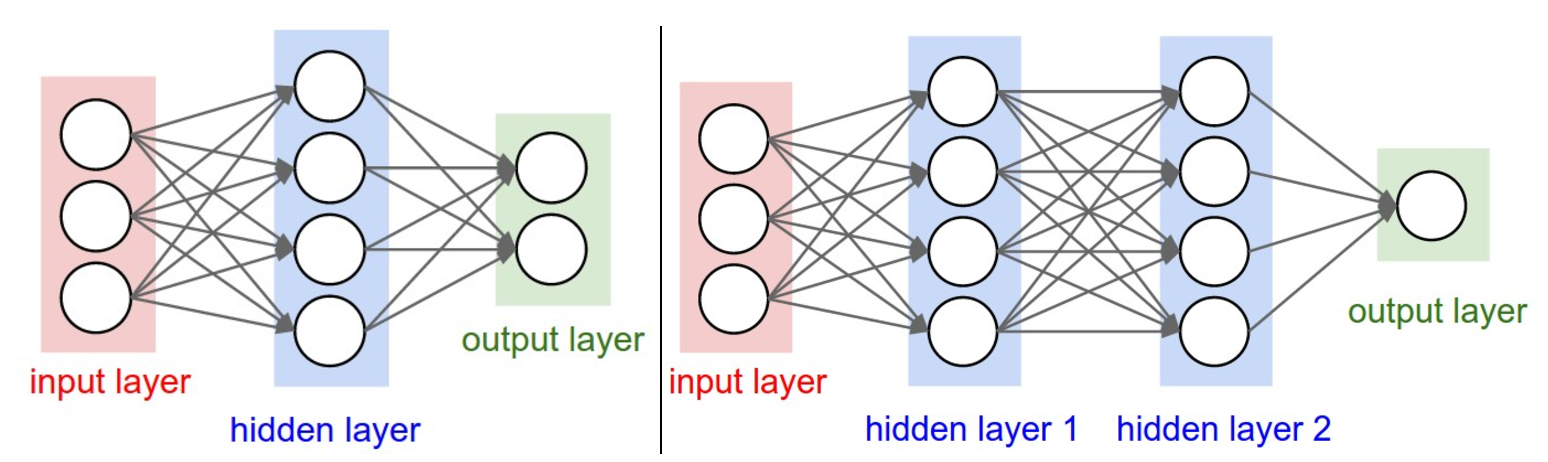
\includegraphics[width=\textwidth]{images/neural_net.png}
\end{figure}
\pv
The key point is that we introduce \textbf{non-linearity between layers}. This non-linearity is often referred to as the \textbf{activation function} (more on this later).
\end{frame}

\begin{frame}{Neural network motivation}
As we've seen several times, linear models do not necessarily fit the data properly. 
\textbf{Example}:
\begin{itemize}
	\item \texttt{AND}, \texttt{OR} and \texttt{NOT} logic operators are linearly separable
	\item \texttt{XOR} is not linearly separable
\end{itemize}
\pv
\textbf{However}: If we transform the inputs with \texttt{AND} and \texttt{NOT} operators to generate new inputs, then \texttt{XOR} becomes linearly separable.
\end{frame}

\begin{frame}{Theoretical guarantees}
There is an interesting theoretical result that is in favor of neural networks modeling called the \textbf{universal approximation theorem} that states (in a nutshell):
\pv
We can approximate any function by a neural network with a neural network with one hidden layer.
\pv
This tells a lot about how powerful neural networks are. However, this is \textbf{just a theoretical result}. We could think that in practice, we just need to use a neural network with one hidden layer with an arbitrary number of neurons (or units), but this does not give good results. Depending on the application, it can be more efficient to \textbf{stack multiple hidden layers}.
\end{frame}

\begin{frame}{Activation functions}
There one issue with stacking neuron layers: The composition of linear function is still linear, so we don't gain any generalization when doing it.
\pv
The solution for this is to \textbf{introduce non-linearity between layers} ($f$), this is called the \textbf{activation function}.
\begin{figure}
\centering
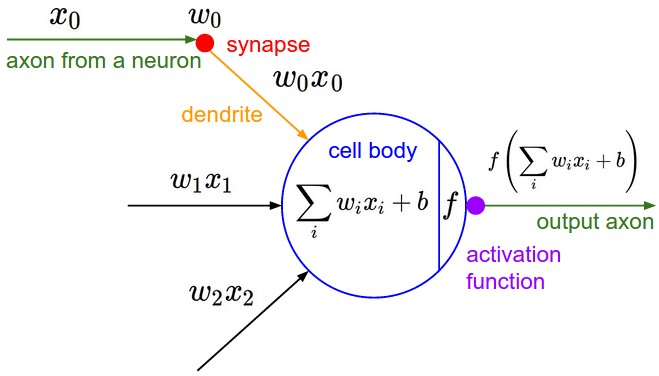
\includegraphics[width=\textwidth]{images/neuron_model.jpeg}
\end{figure}
\end{frame}

\begin{frame}{Activation functions (examples)}
The most commonly used activation functions are:
\begin{itemize}
	\item The \textbf{rectified linear unit (ReLU)}:
	$$ f(x) = \max(0, x)$$
	\pv
	\item The \textbf{logistic sigmoid}:
	$$ f(x) = \dfrac{1}{1 + e^{-x}}$$
	\pv
	\item The \textbf{hyperbolic tangent}:
	$$ f(x) = \tanh(x) = \dfrac{e^x - e^{-x}}{e^x + e^{-x}}$$
\end{itemize}
\pv
With the activation functions, we break the linearity between layers, which leads to richer function representations.
\end{frame}

\begin{frame}{Application: Convolutional neural networks}
Neural networks got a lot of attention thanks to their results in image processing/computer vision. 
\pv
The architecture is a bit different in this case. In images, there is \textbf{a notion of neighborhood} that justifies the use of \textbf{convolutional neural networks} (CNN).
\pv
The neural networks we've mentioned so far are \textbf{fully-connected}, which means that between 2 consecutive layers, all the units are connected. For CNNs, many of the connections are missing.
\end{frame}

\begin{frame}{Application: Convolutional neural networks}
A convolution looks like that:
\begin{figure}
\centering
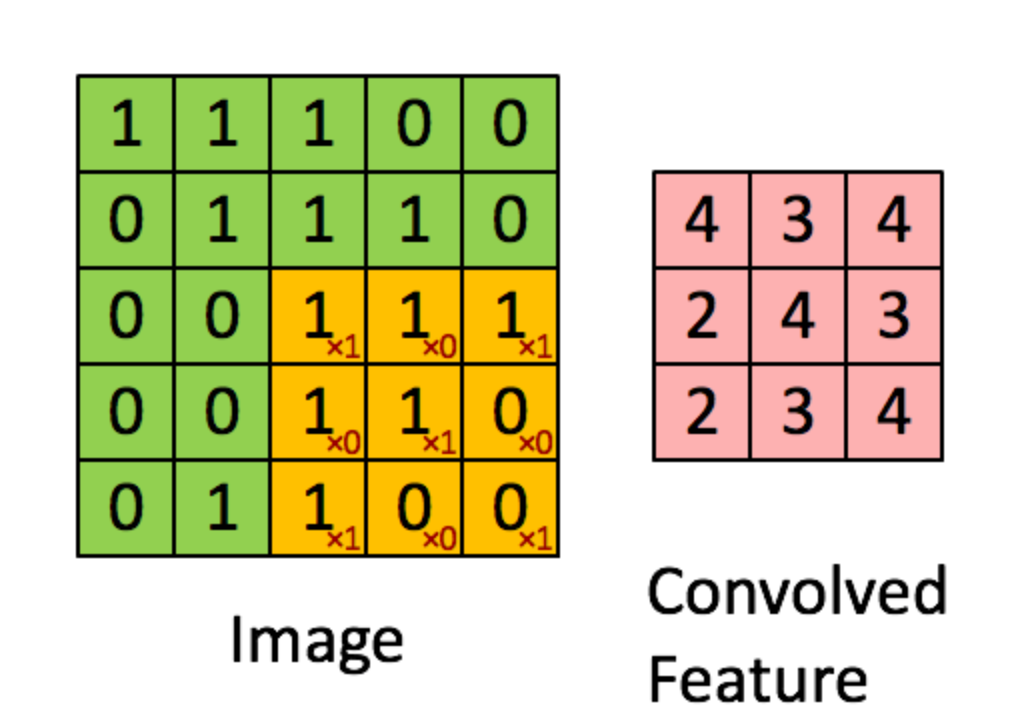
\includegraphics[width=\textwidth]{images/convolution.png}
\end{figure}
\end{frame}

\begin{frame}{Application: Convolutional neural networks}
Convolutions help detect some patterns (e.g. edges) in images:
\pv
\begin{figure}
\centering
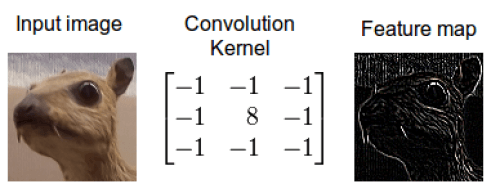
\includegraphics[width=\textwidth]{images/convolution_edge.png}
\end{figure}
\pv
The advantage of CNNs is that they can \textbf{learn the convolutions kernels} and \textbf{find patterns}. We often say that they \textbf{learn features} (as well as learning the model!) for this reason.
\end{frame}

\begin{frame}{Application: Neural auto-encoder}
Auto-encoders are useful for compressing information. They usually have:
\begin{itemize}
	\item An input and an output layer (of course)
	\item A \textbf{hidden layer with a low number of units}
	\item (optional) Other hidden layers to make the model more complex
\end{itemize}
\end{frame}

\begin{frame}{Training neural networks}
So far, we've seen how neural nets are defined. How do we train them?
\pv
In the end, a neural network takes an input $\bx$ and returns an output $\yhat$ that we hope is close enough to $y$. Hence, we can define a loss function (such as the squared loss)
\begin{equation*}
\ell(y, \yhat) = \left( y - \yhat\right)^2.
\end{equation*}
\pv \textbf{The logic is exactly the same} as with linear models:
\begin{itemize}
	\item We define a way to model the output $\yhat$
	\item We chose a loss function $\ell$
	\item We optimize the parameters so that $\yhat \approx y$
\end{itemize}
\pv
The only difference is that a neural network is a more sophisticated way to model the data.
\end{frame}

\begin{frame}{Training neural networks}
To train the model, we can use gradient descent algorithm (as usual). 
\pv
Also, neural networks are \textbf{prone to overfitting} (a lot!), so regularizing them is important. As with other linear models, using an $\ell_2$-norm penalty works well in practice.
\end{frame}

\begin{frame}{Computing the gradient}
Due to stacking layers and having coefficients at each layer, the gradient is a bit harder to compute.
\pv
The method used to compute the gradient and update the weights is the \textbf{backpropagation}. It is based on the chain rule:
$$ \dfrac{\partial f}{\partial x} = \dfrac{d f}{d q} \dfrac{d q}{d x}$$
when we want to compute the derivative of $f(q(x))$.
\end{frame}

\begin{frame}{Conclusions}
Neural networks are very similar to the simpler models we've seen throughout this course. They just rely on a more sophisticated way to model $\yhat$.
\pv
ML algorithm (almost) systematically follow \textbf{the same logic}:
\begin{itemize}
	\item Get some data points $(\bx, y)$
	\item Define a way to model the prediction (e.g. $\theta^T \bx$)
	\item Define a loss function $\ell$
	\item Optimize the loss over the whole training set
\end{itemize}
\end{frame}

\begin{frame}
\begin{center}
\Huge{Thank you! Questions?}
\end{center}
\v
PS: I've updated a few of the notebooks on the GitHub pages. I'll do some more polishing by the end of the week.
\end{frame}

\end{document}